\documentclass[]{memoir}
\title{Problem Set 2}
\author{Brian Fox}
\date{}
\usepackage{enumitem}
\usepackage{geometry}
\geometry{margin=35mm}
\usepackage{graphicx}
\usepackage{multicol}
\begin{document}
\maketitle
\begin{enumerate}
\item \textit{22.1-3} The \textbf{\textit{transpose}} of a directed graph $G=(V,E)$ is the graph $G^{T}=(V,E^{T})$ , where $E^{T}=\{(v,u)\in{}V\times{}V:(u,v)\in{}E\}$. Thus,$G^{T}$ is $G$ with all its edges reversed. Describe efficient algorithms for computing $G^{T}$ from $G$, for both the adjacency-list and adjacency-matrix representations of $G$. Analyze the running times of your algorithms.\vspace{3mm}
\\ 
Adjacency-list($G$)
\begin{enumerate}[label=\arabic*\hspace{2mm}]
\item \textbf{for} each list $L$ in $G$
\item \hspace{1cm} add first element of $L$ to $G^{T}$
\item i = 0
\item \textbf{for} each list $L$ in $G$
\item \hspace{1cm} i = i+1
\item \hspace{1cm} \textbf{for} each element $e$ in $L$
\item \hspace{2cm} \textbf{if} not first element of $e$
\item \hspace{3cm}  append i to $G^{T}$[$e$]
\end{enumerate}
Adjacency-matrix($G$)
\begin{enumerate}[label=\arabic*\hspace{2mm}]
\item r = 1
\item \textbf{while} r $\leq$ rows in $G$
\item \hspace{1cm} c = 1
\item \hspace{1cm} \textbf{while} c $\leq$ columns in $G$
\item \hspace{2cm} $G^{T}(c,r)=G(r,c)$
\item \hspace{2cm} c = c+1
\item \hspace{1cm} r = r+1
\end{enumerate}
\paragraph{}
Adjacency-list($G$) will run $V$ + $E$ iterations which makes it $O(E)$ assuming the graph is connected.  Adjacency-matrix($G$) is $O(V^{2})$
\pagebreak
\item \textit{22.2-4} What is the running time of BFS if we represent its input graph by an adjacency matrix and modify the algorithm to handle this form of input?
\paragraph{}
To queue the connected vertices of the vertex we pop, we will have to iterate over a list of length $V$. This will make the run time $O(V^{2})$
\item \textit{22.3-2} Show how depth-first search works on the graph of Figure 22.6.  Assume that the for loop of lines 5–7 of the DFS procedure considers the vertices in alphabetical order,  and  assume  that  each  adjacency  list  is  ordered  alphabetically.   Show  the discovery and finishing times for each vertex, and show the classification of each edge.
\paragraph{} fig 22.6:
\begin{figure}[h]
	\centering
	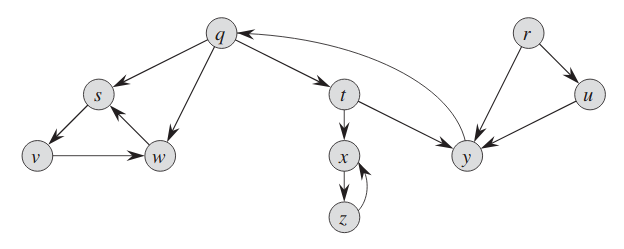
\includegraphics[scale=.5]{fig22-6}
\end{figure}
\begin{multicols}{2}
\begin{enumerate}[label=time \arabic*:]
\item visit q
\item visit s
\item visit v
\item visit w
\item leave w
\item leave v
\item leave s
\item visit t
\item visit x
\item visit z
\columnbreak
\item leave z
\item leave x
\item visit y
\item leave y
\item leave t
\item leave q 
\item visit r
\item visit u
\item leave u
\item leave r
\end{enumerate}
\end{multicols}
\pagebreak
\item \textit{22.3-7} Rewrite the procedure DFS, using a stack to eliminate recursion.
DFS($G$)
\begin{enumerate}[label=\arabic*\hspace{2mm}]
\item \textbf{for} each vertex $u \in G.V$
\item \hspace{1cm} $u.color$ = WHITE
\item \hspace{1cm} $u.\pi$ = NIL 
\item time = 0
\item \textbf{for} each vertex $u \in G.V$
\item \hspace{1cm} \textbf{if} $u.color$ == WHITE
\item \hspace{2cm} DFS-VISIT($G,u$) 
\end{enumerate}
DFS-Visit($G,u$)
\begin{enumerate}[label=\arabic*\hspace{2mm}]
\item time = time + 1
\item $u.d$ = time
\item $u.color$ = GRAY
\item $S$ = Stack(G)
\item \textbf{while} $S$ is not empty
\item \hspace{1cm} \textbf{for} each $v \in G.Adj[u]$
\item \hspace{2cm} \textbf{if} $v.color$ == WHITE 
\item \hspace{3cm} $v.\pi$ = $u$
\item \hspace{3cm} $S$.add($v$)
\item \hspace{2cm} $u.color$ = BLACK
\item \hspace{2cm} time = time + 1
\item \hspace{2cm} $u.f$ = time
\end{enumerate} 
\item \textit{22.4-1} Show the ordering of vertices produced by TOPOLOGICAL-SORT when it is run on the dag of Figure 22.8, under the assumption of Exercise 22.3-2.
\paragraph{} fig 22.8:
\begin{figure}[h]
	\centering
	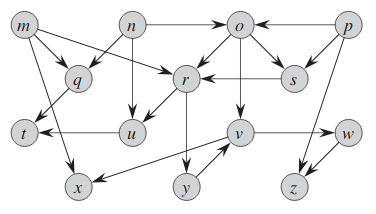
\includegraphics[scale=.5]{fig22-8}
\end{figure}
\paragraph{}
$$p \to n \to o \to s \to m \to r \to y \to v \to x \to w \to z \to u \to q \to t$$
\pagebreak
\item \textit{23-4} In this problem, we give pseudocode for three different algorithms. Each one takes a connected graph and a weight function as input and returns a set of edges $T$. For each algorithm, either prove that $T$ is a minimum spanning tree or prove that $T$ is not a minimum spanning tree. Also describe the most efficient implementation of each algorithm, whether or not it computes a minimum spanning tree.
\begin{enumerate}
\item Maybe-MST-A $(G,w)$ 
\begin{enumerate}[label=\arabic*\hspace{2mm}]
\item sort the edges into nonincreasing order of edge weights $w$
\item $T = E$
\item \textbf{for} each edge $e$, taken in nonincreasing order by weight
\item \hspace{1cm} \textbf{if} $T-\{e\}$ is a connected graph
\item \hspace{2cm}$T=T-\{e\}$
\item \textbf{return} $T$
\end{enumerate}
\paragraph{}
T is a MST. By using an adjacency list you need to sort $E$ items while an adjacency matrix would need to sort $V^{2}$ items. the rest of the algorithm is independent of the data structure used since it uses a list of edges to construct the MST.
\item Maybe-MST-B$(G,w)$
\begin{enumerate}[label=\arabic*\hspace{2mm}]
\item $T=\emptyset$
\item \textbf{for} each edge $e$, taken in arbitrary order
\item \hspace{1cm}\textbf{if} $T\cup\{e\}$ has no cycles
\item \hspace{2cm}$T=T\cup\{e\}$
\item \textbf{return} $T$
\end{enumerate}
\paragraph{}
T is a tree but is not a MST. Checking for cycles will be best done with a DFS. the worst case run time with be the same as a BFS but the average will be better if the cycles contain many vertices. 
\item Maybe-MST-C$(G,w)$
\begin{enumerate}[label=\arabic*\hspace{2mm}]
\item $T=\emptyset$
\item \textbf{for} each edge $e$, taken in arbitrary order
\item \hspace{1cm}$T = T\cup\{e\}$
\item \hspace{1cm}\textbf{if} $T$ has a cycle $c$
\item \hspace{2cm}let $e'$ be a maximum-weight edge on $c$
\item \hspace{2cm}$T=T-\{e'\}$
\item \textbf{return} $T$
\end{enumerate}
\paragraph{}
T is not necessarily a MST or a tree. 
\end{enumerate}
\end{enumerate}
\end{document}
